
In the following chapter, we will discuss shape representation in computer graphics. Explore some of their properties and what tools can be used to modify them. Some of the usual data structures to represent a geometric shape and position within a 3D space are:

\begin{itemize}
    \item \textbf{Mesh} is a set of vertices, edges, and faces defining a 3D object. It is especially used in computer graphics, and it is a simple way to represent complex 3D shapes. A face is a polygon with a minimum of 3 vertices. The most commonly used is a triangle. If a face is made of 4 vertices, it is called a quad, and more than four is called a general polygon. In our case, when we mention faces, we will have triangles in mind. These faces then form a general surface. 
    \begin{figure}[h]
        \centering
        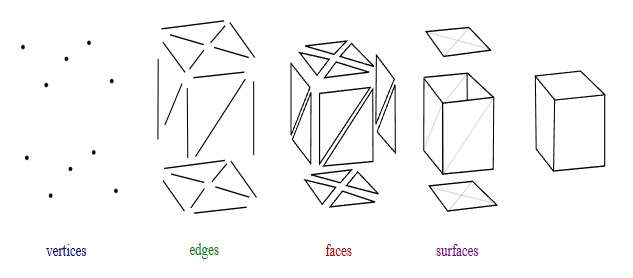
\includegraphics[width=11cm]{mesh.png}
        \caption{Elements of mesh object \cite{stanford}}
        \label{fig:mesh}
    \end{figure}
    
    A 3D object can have a color. To do so, we assign color values to every vertex of the 3D object. The pixel color of the triangle is determined based on the three vertices by which it is made.
    
    \begin{figure}[h]
        \centering
        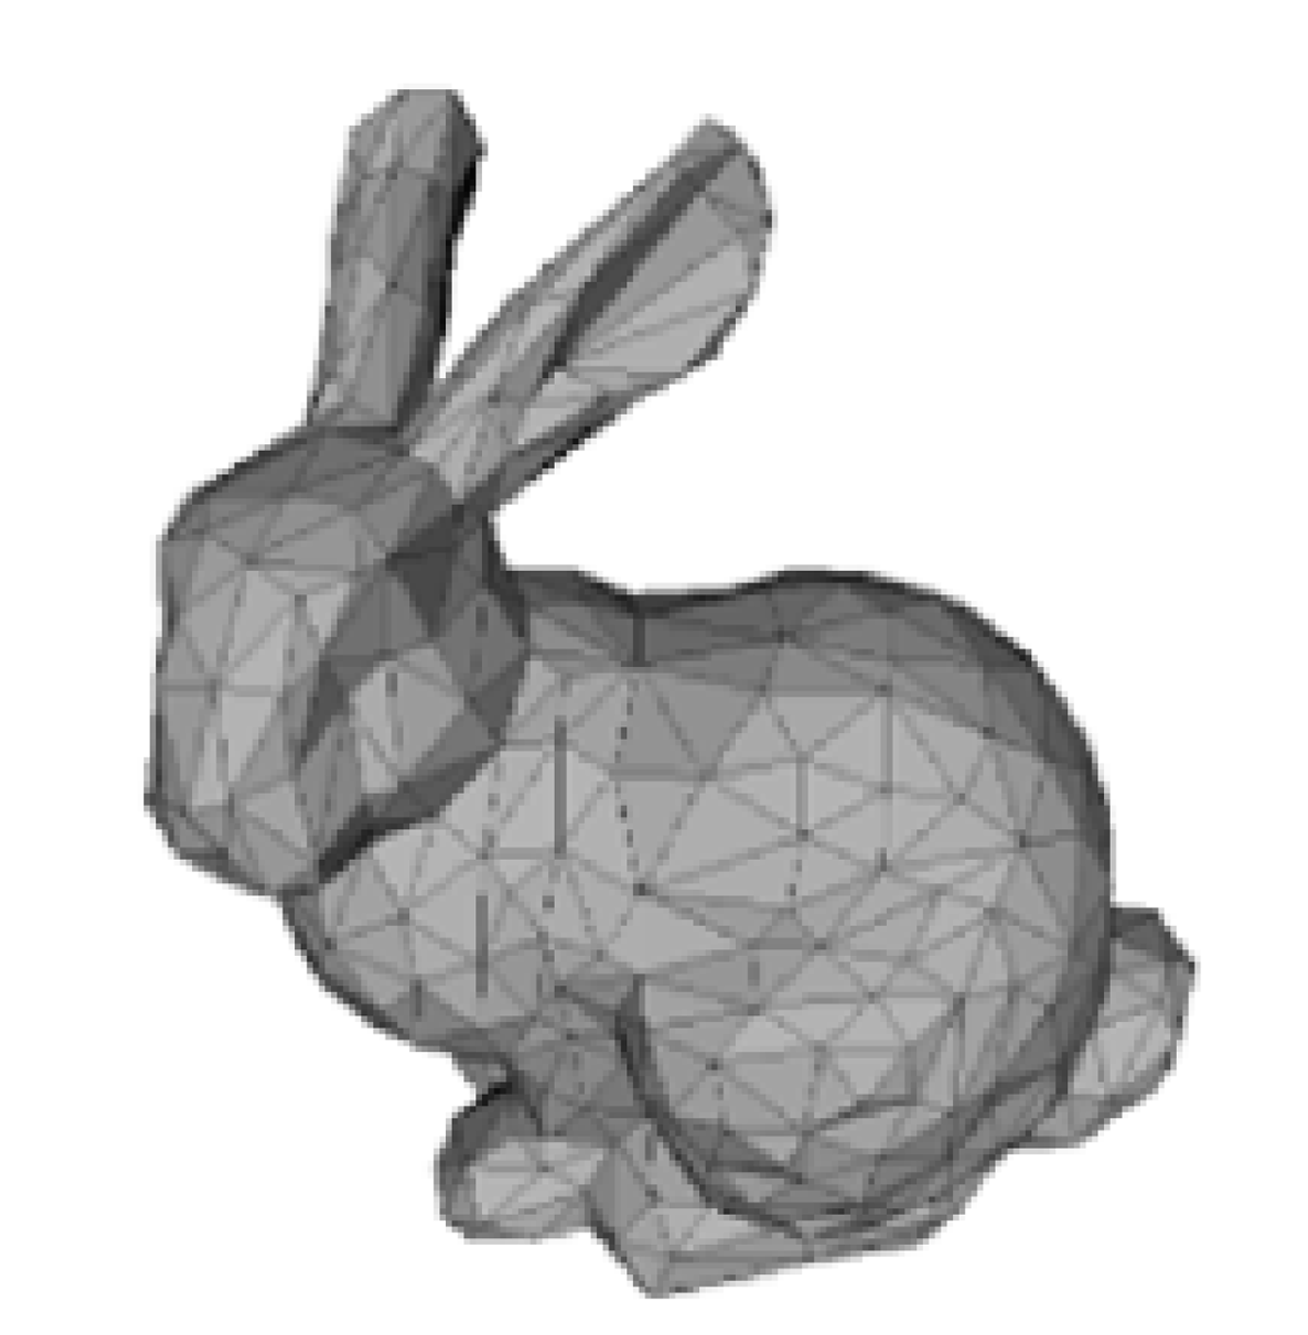
\includegraphics[width=4cm]{rabbit_mesh.png}
        \caption{Stanford bunny model made of mesh \cite{stanford}}
        \label{fig:rabbit_mesh}
    \end{figure}

    \item \textbf{Voxel} objects are in comparison with mesh objects solid. As already said, mesh objects are created from a surface of little triangles, but it is also worth noting that this object is hollow, just like a ballooon. On the other hand, if a model is created from voxels, abbreviation from volumetric pixels, it means that the object was created from cubes and the object itself is solid, its inside also holds information. The working scene is a 3D grid, and its data point holds information about opacity, color, and material information is often also stored.
    
    \begin{figure}[h]
        \centering
        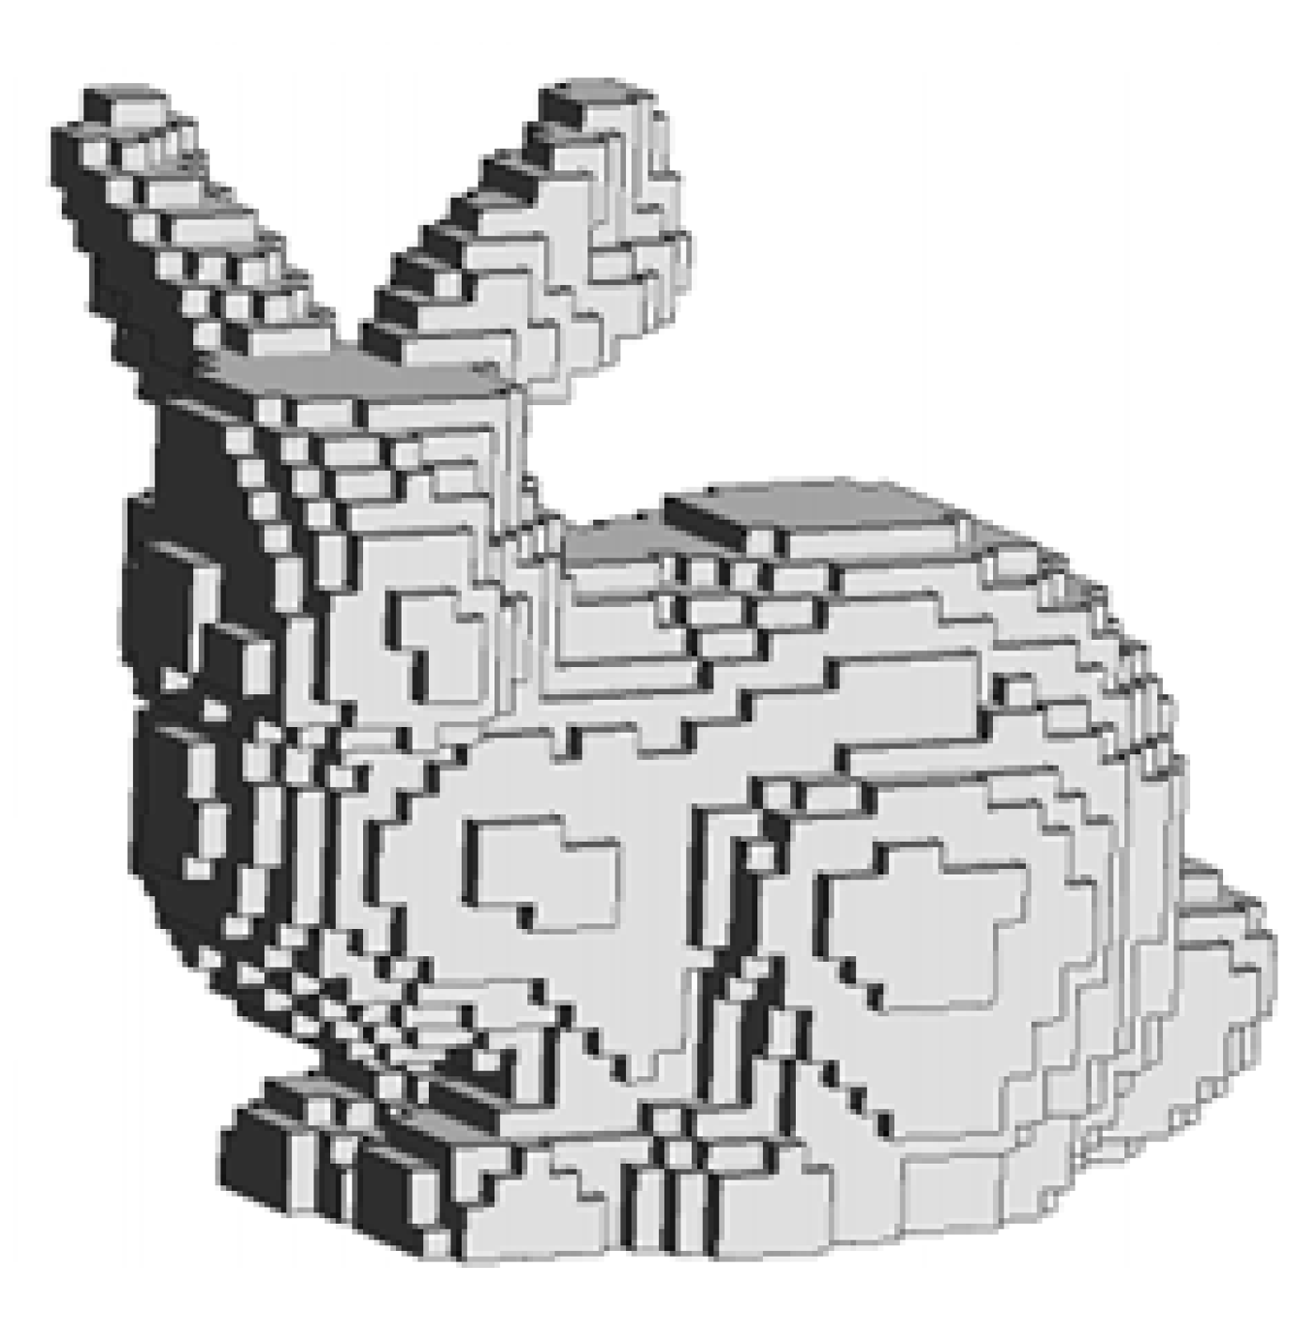
\includegraphics[width=4cm]{rabbit_voxel.png}
        \caption{Stanford bunny model made of voxels \cite{lstmcell_img}}
        \label{fig:rabbit_voxel}
    \end{figure}

    Voxels are often used in medicine and terrain representation. Voxel terrain can represent overhangs, caves, arches, and other, which is difficult to represent using heightmaps, which represents only top-layer data, and anything below it would be filled with no option for holes.

    The main disadvantage of voxels is the resolution. If we want to have a highly detailed voxel model, we would have to increase the resolution of the whole scene.

    \item \textbf{Point cloud} is a collection of points plotted in 3D space. Each point contains position coordinates, color values, and luminance values, determining how bright a point is.
    
    Points are usually acquired by a 3D scanner or photogrammetry software. Scanners work by sending out pulses of light to the object and measuring how long each point takes to reflect back and hit the scanner. These measurements are used to determine the exact positions of points on the object, creating a point cloud. Photogrammetry is a process to create measurements from pictures. It uses photos of an object to triangulate points on the object and plot these points to 3D points, resulting in point clouds.
    
    \begin{figure}[h]
        \centering
        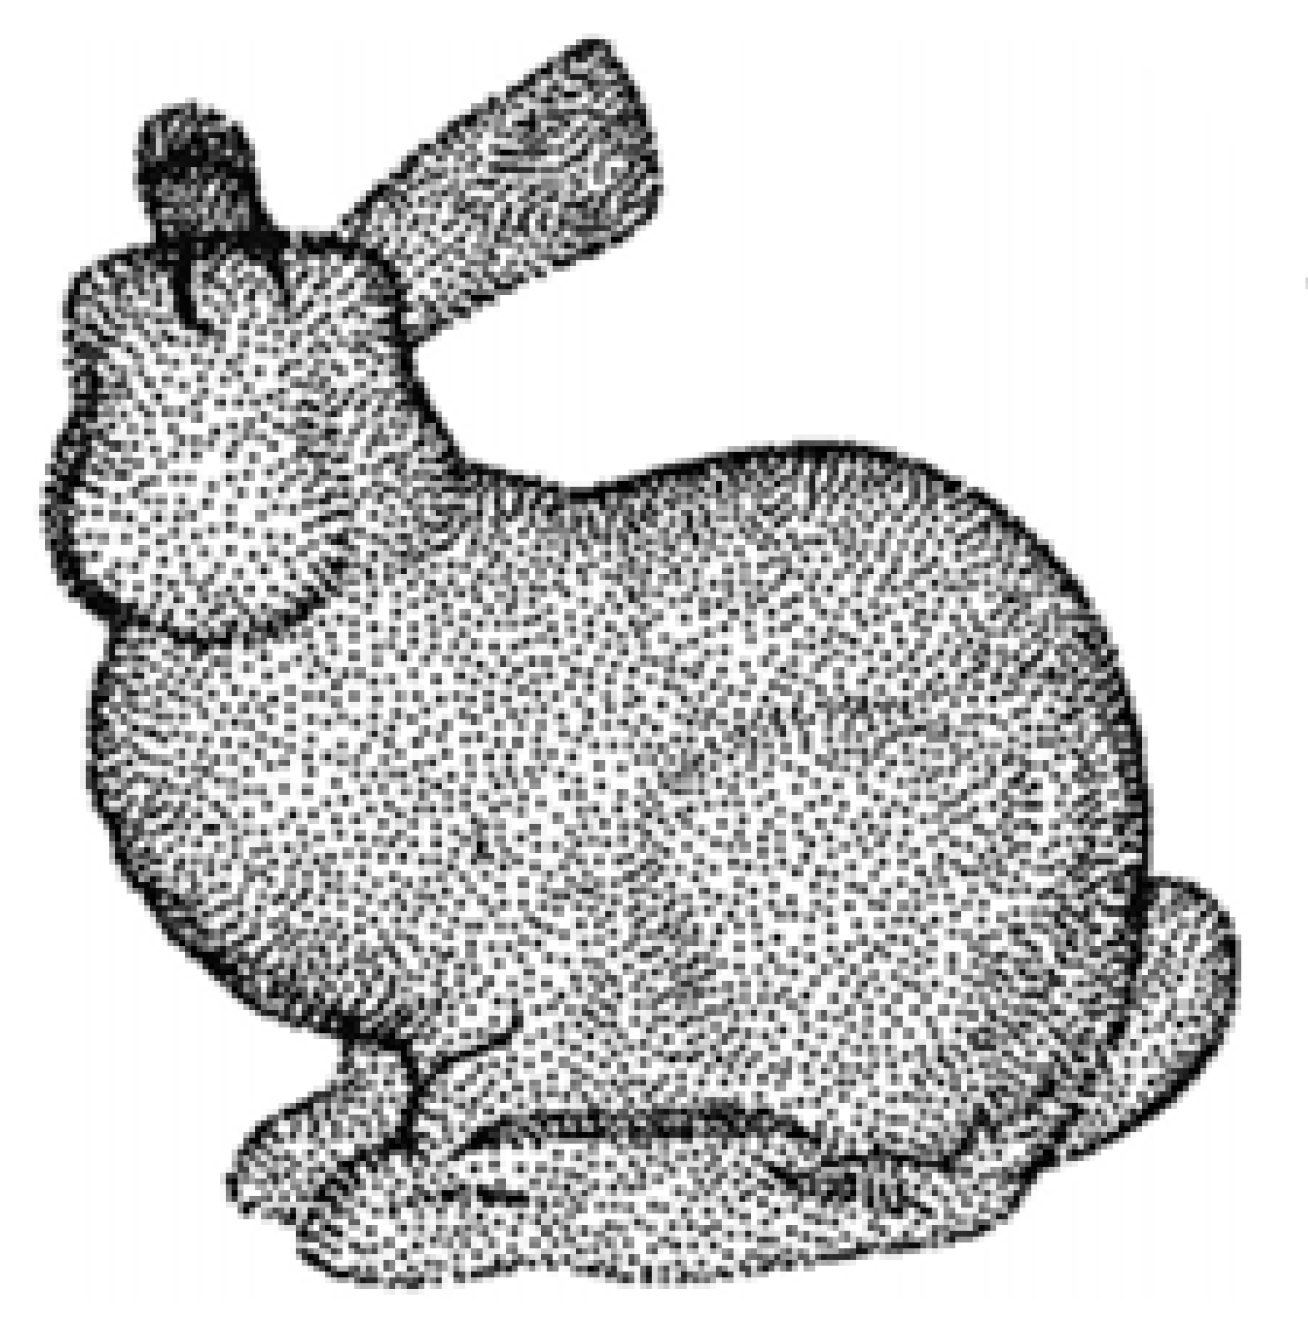
\includegraphics[width=4cm]{rabbit_cloud.png}
        \caption{Stanford bunny model made of point clouds \cite{stnaford}}
        \label{fig:rabbit_cloud}
    \end{figure}
  \end{itemize}

  In terms of the thesis and its goal, we will mainly explore mesh polygons and their edge flow properties while also exploring polygon reduction operations on them.

\section{Edge flow}

Edge flow is a fundamental concept in 3D modeling. The general goal is to ensure that mesh edges follow the curves of an object. A mesh with distinctly different edge flows can represent the same object while preserving the same shape. The key difference and significance of edge flows plays in the world of animation, overall any deformation operation performed on the object. In general, a good edge flow has uniformly distributed points along the 3d model, meaning the length and the area of each primitive is also of similar if not equal sizes. 

\begin{figure}[h]
    \centering
    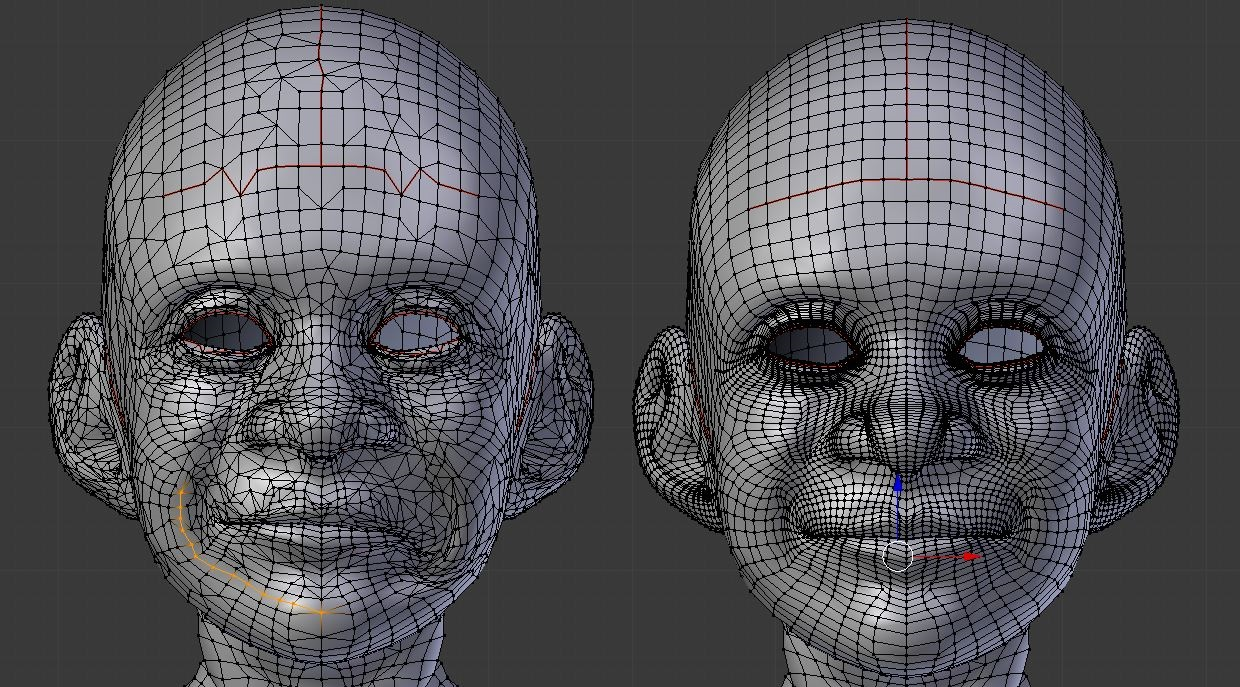
\includegraphics[width=12cm]{topology.png}
    \caption{A mesh object constructed with 2 different edge flows \cite{decimation}}
    \label{fig:topology_comp}
\end{figure}

An optimal edge flow allows smooth and natural deformations. In the case of figure \ref{fig:topology_comp}, if we want to animate various facial expressions, the left example would have distorted wrinkles. In contrast, the right example would allow for natural mimicry, as we are familiar with in real life. A more expressive example would be in \ref{fig:planar_def}, where we can see a plane of two different topologies having different behavior if bent. The left example has slight bumpy artifacts, while the right preserves smooth surface transition.

\begin{figure}[h]
    \centering
    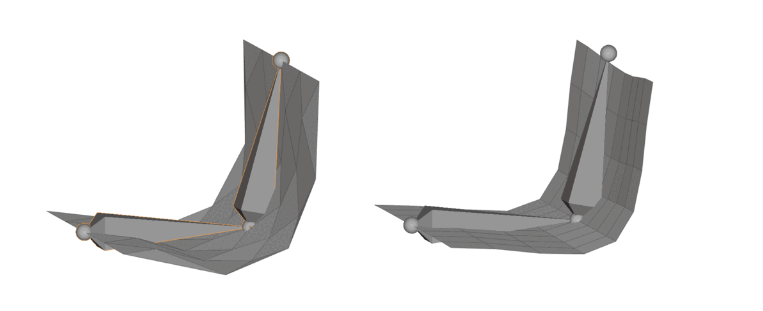
\includegraphics[width=12cm]{planar_deform.png}
    \caption{Deformation of the same object with different edge flow \cite{topology_animation}}
    \label{fig:planar_def}
\end{figure}

Edge flows are manually crafted by 3D artist and require experience to reach their optimal form. They are either being considered from the beginning while creating the 3D mesh or as a post-correction, where the acquired 3D mesh does not meet the required quality needed for future work. One of the possible reasons for having insufficient quality could be caused by polygon reduction.

\section{Polygon reduction}
Polygon reduction is a common practice for performance and memory optimization as a higher number of polygons may introduce greater details, but they also bring high demand on hardware requirements. A high polygon mesh is usually a byproduct of the 3D scanning process where the resulting 3D mesh can be of enormous memory size. Most importantly, the reduced amount should be considered as the reduction can lose the visual representation of the object and its key features. The general goal is to balance visual quality and performance optimization. Following, we will list some of the most used techniques for polygon reduction and their effect on the resulting edge flow. Edge flow is a fundamental concept in 3D modeling, playing a pivotal role in natural 3D model deformations mostly used in animation. 

\section{Decimation}

Decimation is a commonly used method for quick polygon reduction. It reduces the percentage of vertices and edges uniformly while preserving the overall shape of the reduced object, but it does not handle fine details well. Most 3d modeling software, such as Blender, Maya, 3ds Max, Zbrush, and Cinema4D, support decimation since it is a common technique. The overall control or workflow may differ, but the general concept remains the same.\cite{decimation}

\begin{figure}[h]
    \centering
    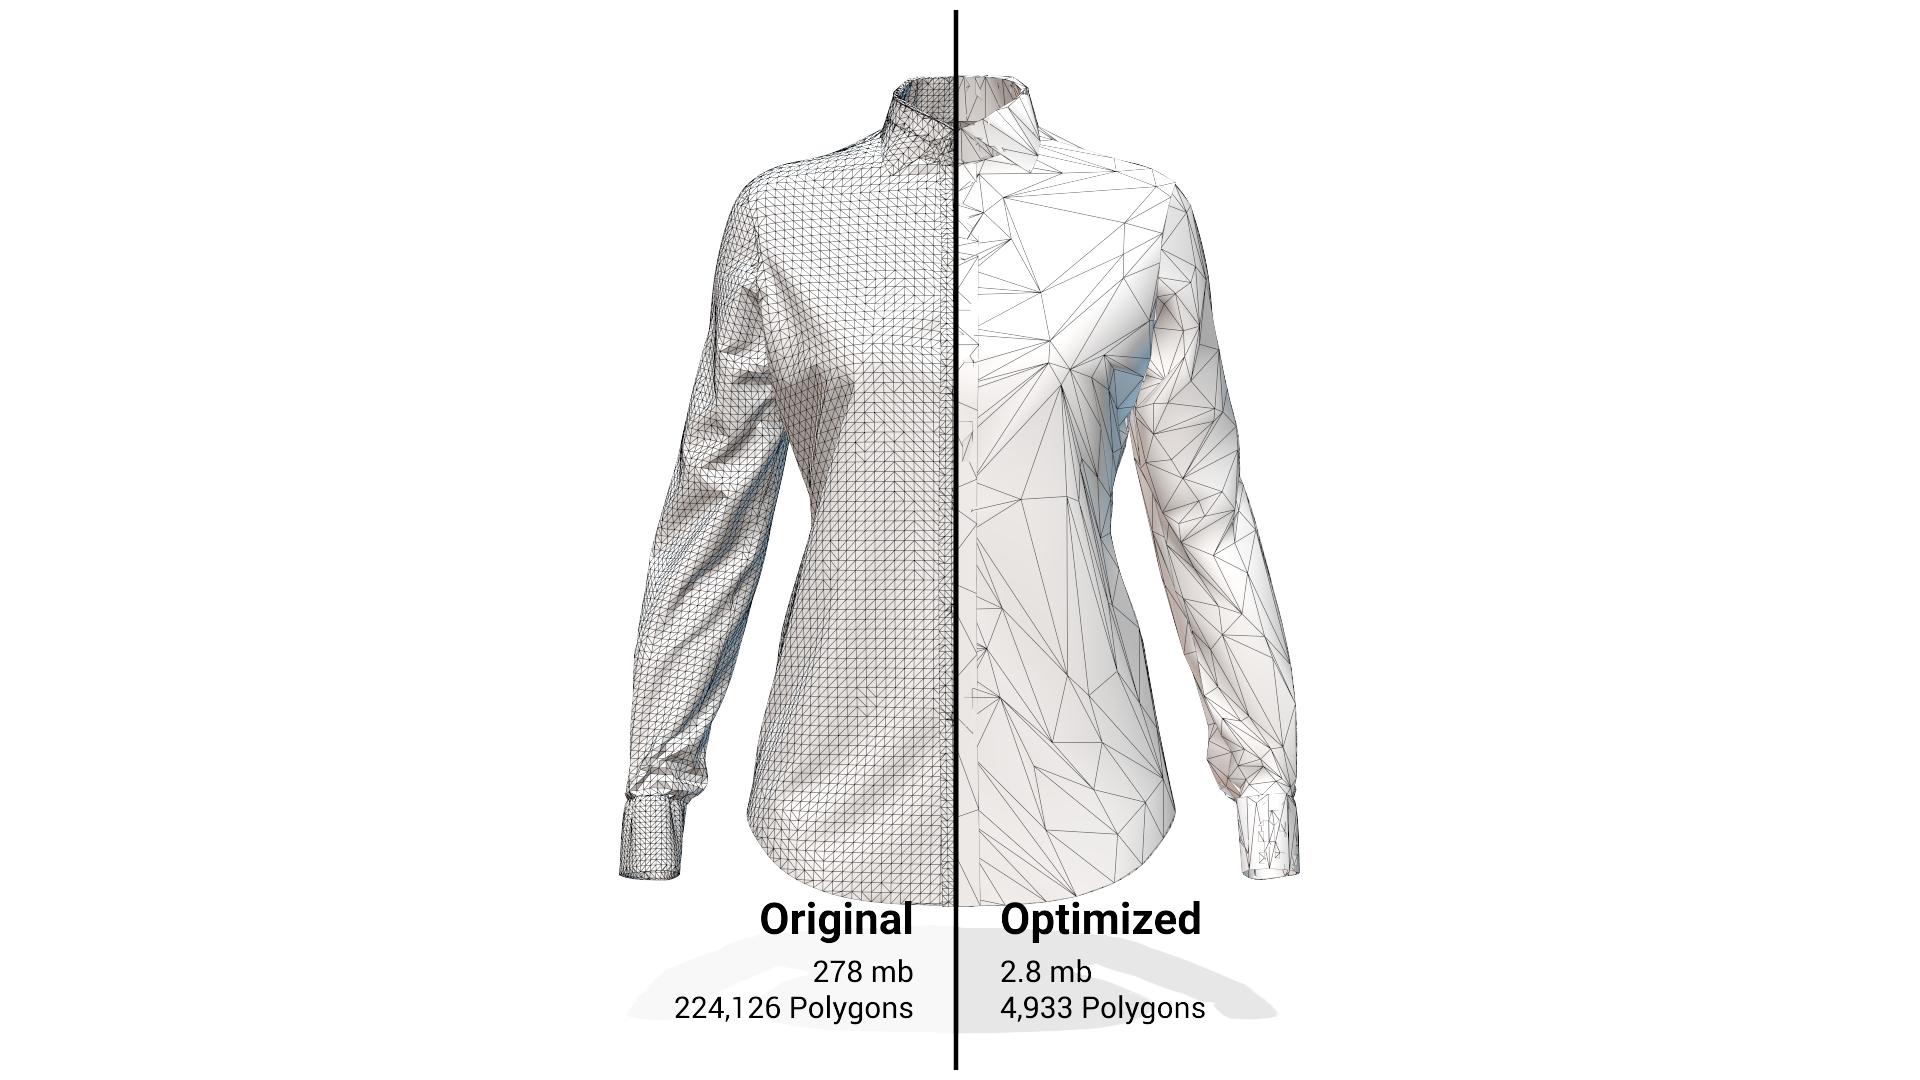
\includegraphics[width=12cm]{ShirtComparison.png}
    \caption{Decimation applied on shirt 3D mesh \cite{decimation}}
    \label{fig:shirt_comp}
\end{figure}

As seen in \ref{fig:shirt_comp}, the optimized 3D mesh may be optimized in the number of polygons, but its edge flow suffered greatly. If the shirt was part of any animated object, its part would deform unnaturally in undesired ways.

\section{Retopology}

Retopology is a semi-automatic method requiring high user input. Retopology requires a user to manually outline the required surface by hand while hinting at its edge flow by following the model's edges before the 3D software follows the outlines and draws a polygon. This gives a user high control over its model but is highly demanding on general experience and skill while identifying the edges. From a quality perspective, the resulting model will be suitable for animations and smooth 3D model deformations. Still, from a workflow efficiency standpoint, producing one of these reduced models requires a lot of time.

\begin{figure}[h]
    \centering
    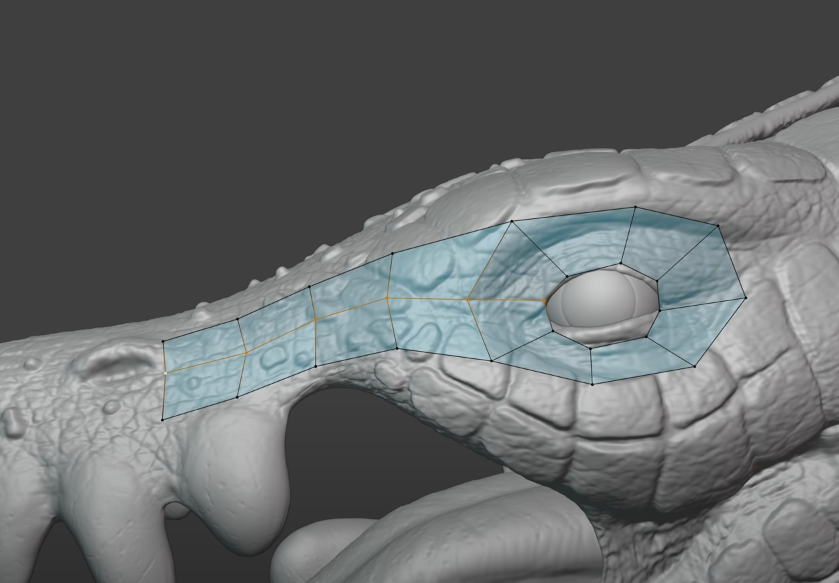
\includegraphics[width=12cm]{retopology.png}
    \caption{Retopology surface manually created lizard 3D mesh \cite{retopology}}
    \label{fig:retopology}
\end{figure}

\section{Quad Remeshing}

Instant remesh

Eh...

Decimation -> automatic reduction
Decimation does not preserve edge flow

* polygon reduction tools
* retopology -> requires manual work Blender
* quad remeshing -> often use to preserve nice deformation -> for animation -> main nemesis
* edge collapse -> manual work

These reduction techniques don't ensure so called edge flow, a fundamental concept in 3D modeling playing a pivotal role in natural 3D model deformation mostly used in animation.